% !TEX program = xelatex
\documentclass[letterpaper]{article}
\usepackage[margin=0.45in]{geometry}
\usepackage{fontspec}
\usepackage{amsmath}
\usepackage{xcolor}
\usepackage{graphicx}
\usepackage{listings}
\usepackage[most]{tcolorbox}

\setmainfont{Menlo}
\setmonofont{Menlo}

\definecolor{background}{HTML}{0D0D14}
\definecolor{surface}{HTML}{181B25}
\definecolor{text}{HTML}{CFD6E4}
\definecolor{heading}{HTML}{F4F6FB}
\definecolor{muted}{HTML}{8D95A8}
\definecolor{accent}{HTML}{F2C14E}

\pagecolor{background}
\color{text}
\pagestyle{empty}
\setlength{\parindent}{0pt}
\AtBeginDocument{\raggedright}
\setlength{\parskip}{0.7em}
\linespread{1.25}
\renewcommand{\normalsize}{\fontsize{9}{11.5}\selectfont}

\graphicspath{{figures/}}

\newcommand{\heading}[1]{\par\vspace{0.4em}{\fontsize{10.5}{13}\selectfont\bfseries\color{heading}#1}\par\vspace{0.1em}}
\newcommand{\code}[1]{{\setlength{\fboxsep}{1pt}\colorbox{surface}{\textcolor{accent}{\detokenize{#1}}}}}
\newcommand{\figcaption}[1]{\par\vspace{0.4em}{\centering\fontsize{8}{10.5}\selectfont\color{muted}#1\par}}

\lstset{
  basicstyle=\fontsize{8.2}{10.8}\selectfont\ttfamily\color{accent},
  columns=fullflexible, keepspaces=true, showstringspaces=false,
}

\newtcblisting{codeblock}{listing only, colback=surface, colframe=surface, coltext=accent, boxrule=0pt, arc=0pt,
  left=6pt, right=6pt, top=3pt, bottom=3pt, before skip=0.5em, after skip=0.7em}

\newtcolorbox{eqbox}{enhanced, colback=surface, colframe=accent, boxrule=0pt, leftrule=2pt, arc=0pt,
  left=6pt, right=6pt, top=1pt, bottom=1pt, before skip=0.4em, after skip=0.6em, fontupper=\color{heading}}
\newtcolorbox{figbox}{colback=surface, colframe=surface, boxrule=0pt, arc=0pt, left=6pt, right=6pt, top=6pt, bottom=6pt,
  before skip=0pt, after skip=0pt}

\newenvironment{textcol}[1]{\begin{minipage}[t]{#1\linewidth}\vspace{0pt}\raggedright\setlength{\parskip}{0.7em}}{\end{minipage}}
\newcommand{\figcol}[2]{\begin{minipage}[t]{#1\linewidth}\vspace{0pt}\begin{figbox}#2\end{figbox}\end{minipage}}

\begin{document}



\vspace{1.4em}
\begin{textcol}{0.54}
\heading{Building the ribbon}
To turn the saved positions into a ribbon, each one gets a vertex on either side of the path. The side
direction is perpendicular to the way the ball was moving there, which we get from the two neighboring points:
\begin{eqbox}
\[
  \mathbf p_i^\pm = \mathbf p_i \pm w_i\,\hat{\mathbf n}_i,
  \qquad w_i = 0.4\,(1-a_i),
  \qquad a_i = \frac{i}{39}
\]
\end{eqbox}
Here $\mathbf p_i$ is a saved position with $i = 0$ the newest, and $\hat{\mathbf n}_i$ is the unit vector
perpendicular to the path. $a_i$ is the age of the point, from 0 at the ball to 1 at the tail, so the
half-width $w_i$ shrinks from 0.4 to 0 and the ribbon tapers to a point.
\end{textcol}\hfill
\figcol{0.42}{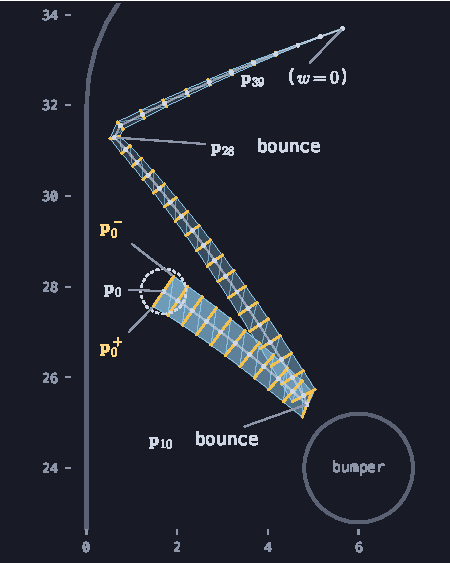
\includegraphics[width=\linewidth]{fig_ribbon.pdf}
  \figcaption{The same 40 points in table space. Gold rungs connect each $\mathbf p_i^+$ to $\mathbf p_i^-$, and
  the dashed circle is the ball. Where the ball reverses at the bumper, the ribbon twists through a point.}}

The perpendicular is the direction of travel, $\mathbf p_{i-1} - \mathbf p_{i+1}$, rotated $90^\circ$ by
swapping its components and negating one, then divided by its length. The ends of the array reuse their one
neighbor. The vertices go into a buffer in the order $\mathbf p_0^+, \mathbf p_0^-, \mathbf p_1^+,
\mathbf p_1^-, \ldots$, which is what \code{gl.TRIANGLE_STRIP} wants, and every pair is lifted a little above
the playfield so the ribbon doesn't z-fight with it.
\begin{codeblock}
trail.forEach(([x, y], i) => {
  const [ax, ay] = trail[Math.max(i - 1, 0)];
  const [bx, by] = trail[Math.min(i + 1, trail.length - 1)];
  const len = Math.hypot(ax - bx, ay - by) || 1;
  const age = i / (TRAIL_LENGTH - 1);
  const w = TRAIL_WIDTH * (1 - age);
  const nx = -(ay - by) / len * w;
  const ny = (ax - bx) / len * w;
  trailPositions.set([x + nx, y + ny, TRAIL_HEIGHT,
                      x - nx, y - ny, TRAIL_HEIGHT], i * 6);
  trailTexCoords.set([age, 1, age, -1], i * 4);
});
\end{codeblock}

\vspace{0.8em}
\begin{textcol}{0.54}
\heading{Fading and glow}
Each vertex also gets a texture coordinate: \code{x} is its age $a$, and \code{y} is its side $s$, which runs
from $-1$ at one edge through 0 in the middle to $+1$ at the other edge. The fragment shader turns those into a
brightness:
\begin{eqbox}
\[
  \mathbf C(a, s) = \mathbf C_{\text{trail}}\,(1 - s^2)\,(1 - a)^2
\]
\end{eqbox}
\begin{codeblock}
float fade = 1.0 - vTexCoord.x;
float core = 1.0 - vTexCoord.y * vTexCoord.y;
fragColor = vec4(uColor * core * fade * fade, 1.0);
\end{codeblock}
So the streak is brightest down the middle and at the ball, dark at the edges, and fades toward the tail.
Halfway down the trail the middle is a quarter as bright as the head.
\end{textcol}\hfill
\figcol{0.42}{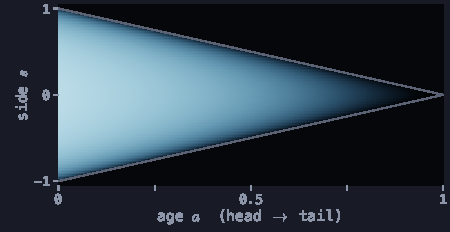
\includegraphics[width=\linewidth]{fig_glow_plain.pdf}
  \figcaption{The ribbon unrolled: brightest at the head and along the middle.}}


\vspace{1.4em}
\begin{textcol}{0.54}
\heading{How fast the flipper is moving}
Every substep the ball is tested against the flipper's centerline, the segment from its pivot to its tip.
$\mathbf q$ is the point on that segment closest to the ball, and $\mathbf r$ points from the pivot to
$\mathbf q$. Because the flipper turns about its pivot, $\mathbf q$ moves perpendicular to the flipper:
\begin{eqbox}
\[
  \mathbf v_s = \omega\,(-r_y,\; r_x),
  \qquad
  \lVert \mathbf v_s \rVert = |\omega|\,\lVert \mathbf r \rVert
\]
\end{eqbox}
$\omega$ is the flipper's angular velocity. The speed grows with distance from the pivot, so contact near the
tip can give a stronger hit. A rising flipper turns at 18~rad/s, so its tip, 3.2 units out, moves at almost
58~units/s.
\end{textcol}\hfill
\figcol{0.42}{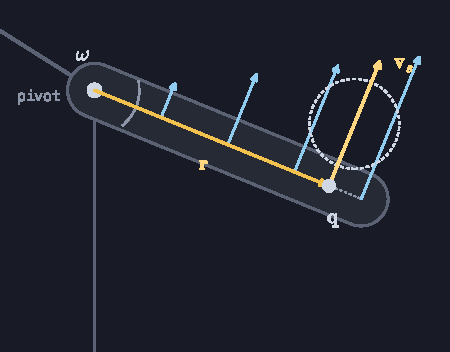
\includegraphics[width=\linewidth]{fig_speed.pdf}
  \figcaption{Blue arrows show how fast each part of the flipper moves; $\mathbf v_s$ is the velocity at the
  contact point.}}

In code, \code{collideFlippers()} works out $\mathbf q$, $\mathbf r$ and $\mathbf v_s$ for each flipper and
hands them to \code{resolve()}, along with the contact distance (ball radius plus flipper radius) and the
flipper's restitution of 0.3:
\begin{codeblock}
function collideFlippers(ball) {
  for (const f of table.flippers) {
    const q = closestOnSegment(ball.p, f.pivot, flipperTip(f));
    const r = sub(q, f.pivot);
    const vs = [-f.omega * r[1], f.omega * r[0]];
    resolve(ball, q, BALL_RADIUS + f.radius, 0.3, vs);
  }
}
\end{codeblock}

\vspace{0.8em}
\begin{textcol}{0.54}
\heading{The bounce}
\code{resolve()} takes $\mathbf n$, the unit vector from $\mathbf q$ toward the ball, and pushes the ball out
of the flipper along it. If the ball and the flipper surface are moving toward each other along $\mathbf n$, it
reverses that part of the ball's velocity, measured relative to the moving surface:
\begin{eqbox}
\[
  \mathbf v_{\text{out}} = \mathbf v_{\text{in}}
  - 1.3\,\big[(\mathbf v_{\text{in}} - \mathbf v_s)\cdot\mathbf n\big]\,\mathbf n
\]
\end{eqbox}
This only happens when the dot product is negative. The 1.3 is $1 + e$, with the flipper's restitution
$e = 0.3$.
\end{textcol}\hfill
\figcol{0.42}{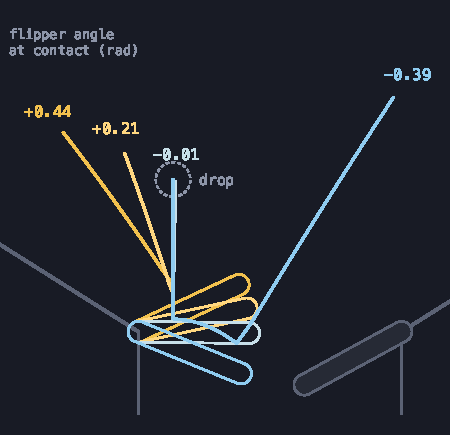
\includegraphics[width=\linewidth]{fig_fan.pdf}
  \figcaption{The later the flip, the lower the flipper and the further right the shot.}}

\vspace{0.6em}
\begin{codeblock}
function resolve(ball, q, reach, restitution, vs = [0, 0]) {
  const d = sub(ball.p, q);
  const dist = Math.hypot(d[0], d[1]);
  if (dist >= reach || dist === 0) return false;
  const n = [d[0] / dist, d[1] / dist];
  ball.p[0] += n[0] * (reach - dist);
  ball.p[1] += n[1] * (reach - dist);
  const vn = dot(sub(ball.v, vs), n);
  if (vn < 0) {
    ball.v[0] -= (1 + restitution) * vn * n[0];
    ball.v[1] -= (1 + restitution) * vn * n[1];
  }
  return true;
}
\end{codeblock}
So the shot comes from the moment of contact. Pressing earlier or later changes the flipper's angle when it
meets the ball, which changes $\mathbf n$ and the direction the ball leaves in.

The flipper's material has a dark ordinary color and uses the palette color as its emissive term, which adds
brightness directly, even where the lights leave the surface dark. \code{draw()} scales it by the brightness and
sends it to the shader:
\begin{codeblock}
flipper: { color: [0.1, 0.1, 0.1], ks: 0.4, shininess: 40, emissive: palette.flipper },

draw(flipperMesh, multiply(frame, translate(0, 0, 0.25), scale(1, 1, h - 0.25)),
     MATERIALS.flipper, f.pressed ? 1.6 : 1);

gl.uniform3fv(uniforms.uEmissive, (mat.emissive ?? BLACK).map(v => v * boost));
\end{codeblock}
The fragment shader adds the emission to the ordinary lighting. For the flipper \code{uTopEmissive} is zero, so
this is just \code{result += emission}, and the flipper comes out bright but sharp-edged:
\begin{codeblock}
result += emission + uTopEmissive * smoothstep(0.7, 0.9, dot(N, uUp));
\end{codeblock}

\vspace{0.8em}
\heading{Bloom}
The bloom pass keeps only the brightness above a threshold of 1 and blurs it horizontally and vertically. It
repeats that over four smaller and smaller images, which gives both a narrow and a wide glow. The final shader
adds the blur back to the scene:
\begin{eqbox}
\[
  \mathbf H = 1.4\,\big(\mathbf S + 0.35\,\mathbf B\big)
\]
\end{eqbox}
$\mathbf S$ is the original scene and $\mathbf B$ is the combined blur, before the final display conversion.

\begin{figbox}

\includegraphics[width=0.327\linewidth]{bloom_scene.jpg}\hfill
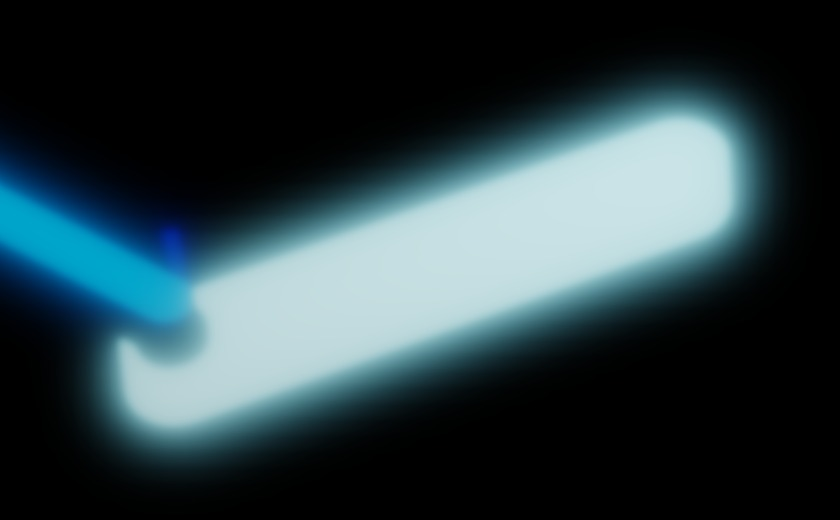
\includegraphics[width=0.327\linewidth]{bloom_bloom.jpg}\hfill
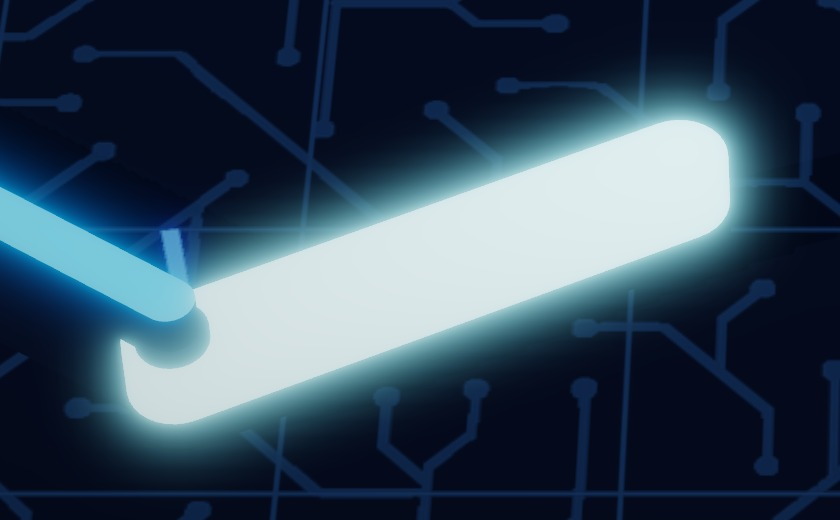
\includegraphics[width=0.327\linewidth]{bloom_full.jpg}
\figcaption{Left: the scene. Middle: the blurred bright parts. Right: the two combined.}
\end{figbox}

\begin{codeblock}
return max(texture(uImage, uv).rgb - uThreshold, 0.0);

vec3 hdr = EXPOSURE * (texture(uScene, vUv).rgb + BLOOM_STRENGTH * bloom);
\end{codeblock}
Pressing a flipper raises its emission, which gives the bloom more brightness to spread around its edges. 

\end{document}
